\documentclass[xcolor={dvipsnames},screen, aspectratio=43,compress]{beamer}
\usepackage[T1]{fontenc}
\usepackage[utf8]{inputenc}

\usepackage{textcomp}
\usepackage{lmodern}

\usepackage{tikz}
\usetikzlibrary{arrows.meta,arrows}
\usetikzlibrary{calc}
\usetikzlibrary{positioning}

\usepackage[subpreambles,mode=image]{standalone}
\usepackage[absolute,overlay]{textpos}
\usepackage{amsthm}
\usepackage{mathtools}
\usepackage{bm}
\usepackage[normalem]{ulem}

\newcommand\redout{\bgroup\markoverwith
{\textcolor{red}{\rule[0.5ex]{2pt}{1pt}}}\ULon}


\renewcommand\Longrightarrow{%
 \mathrel{%
  \mbox{\fontfamily{cmr}\fontencoding{OT1}\selectfont=}}%
 \joinrel\Rightarrow}



%\usepackage{my_commands}
\providecommand{\adv}{\mathbf{Adv}}
\providecommand{\protocol}{\Pi}
\providecommand{\protocolderived}{\protocol^{+}}
\providecommand{\oracle}[1]{\pi_{\hspace*{-1pt}#1}}
\providecommand{\concat}{\Vert}
\providecommand{\A}[1][A]{\mathcal{#1}}
\providecommand{\dlog}[2]{\textcolor{#1}{#2}}
\providecommand{\ua}[1]{\dlog{red}{#1}}
\providecommand{\ub}[1]{\dlog{blue}{#1}}
\providecommand{\uc}[1]{\dlog{Plum}{#1}}
\providecommand{\ud}[1]{\dlog{OliveGreen}{#1}}


\usetheme[style=horizontal,language=en]{ntnu2017}


\newcount\mycount
\renewcommand\includestandalone[2][]{%
    \begingroup
    \pdfximage{#2.pdf}%
    \chardef\npages\pdflastximagepages\relax
    \mycount=1 %
    \loop
        \includegraphics<\the\mycount>[page=\mycount,#1]{#2.pdf}%
        \ifnum\mycount<\npages %
        \advance\mycount by 1 %
    \repeat
    \endgroup
}

\makeatletter
\let\beamer@writeslidentry@miniframeson=\beamer@writeslidentry
\def\beamer@writeslidentry@miniframesoff{%
  \expandafter\beamer@ifempty\expandafter{\beamer@framestartpage}{}% does not happen normally
  {%else
    % removed \addtocontents commands
    \clearpage\beamer@notesactions%
  }
}
\newcommand*{\miniframeson}{\let\beamer@writeslidentry=\beamer@writeslidentry@miniframeson}
\newcommand*{\miniframesoff}{\let\beamer@writeslidentry=\beamer@writeslidentry@miniframesoff}
\makeatother


\newcommand{\backupbegin}{
   \newcounter{finalframe}
   \setcounter{finalframe}{\value{framenumber}}
}
\newcommand{\backupend}{
   \setcounter{framenumber}{\value{finalframe}}
}



\setbeamertemplate{itemize item}[circle]
\setbeamertemplate{itemize subitem}{--}


\title{A Modular Security Analysis of\\EAP and IEEE~802.11}
\subtitle{PhD defense}
\author{H\aa kon Jacobsen}
\institute{Department of Information Security and\\Communication Technology}
\date{October 25, 2017}



\begin{document}


\begin{frame}
  \titlepage
\end{frame}

\section{Intro}
\subsection{intro}





\begin{frame}<1>[label=KE_example]{IEEE 802.11 -- WPA2-PSK}
	\frametitle<2->{eduroam}
	\begin{figure}
		\includestandalone[width=0.75\textwidth]{tikz_intro_slide}
	\end{figure}
\end{frame}





\begin{frame}{WPA2-Enterprise}
	 \begin{columns}
		 \begin{column}{.49\textwidth}
			\centering
			\begin{itemize}
				\item Used in large organizations 
				
				\begin{itemize}
				\item infeasible to share a single shared key
				
				\item user authentication centrally managed
				\end{itemize}
				
				\item Example: eduroam
				
			\end{itemize}
		\end{column}

		\begin{column}{.50\textwidth}
		   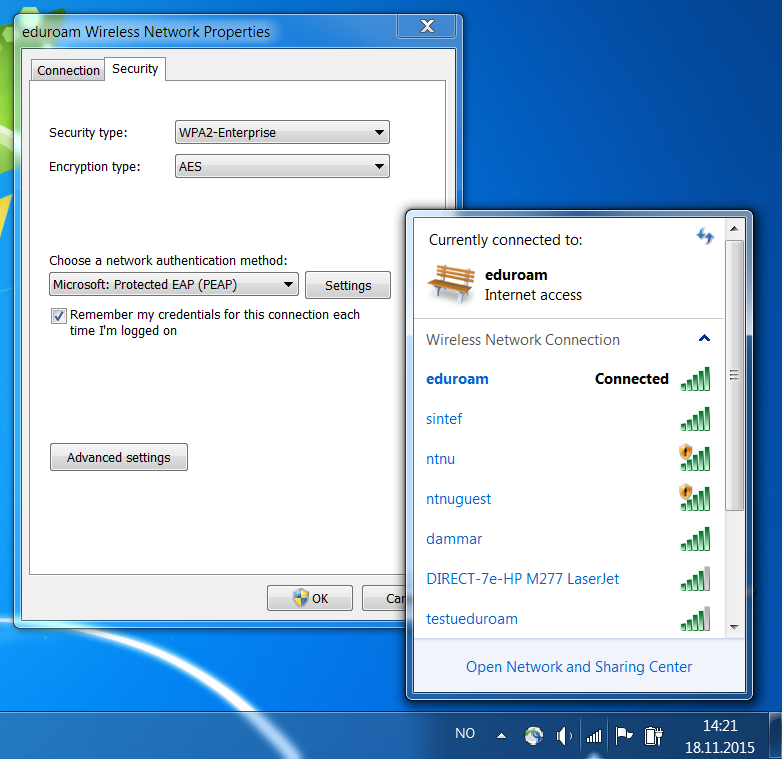
\includegraphics[width=\textwidth]{wireless}
		 \end{column}
	\end{columns}
\end{frame}

%\againframe<3->{KE_example}

\begin{frame}<3>{WPA2-Enterprise}
	\begin{figure}
		\centering
		\includegraphics[page=1,trim={1cm 3cm 1cm 2cm},clip,width=0.95\textwidth]{tikz_EAP_and_802_11}%
	\end{figure}
\end{frame}

%\begin{frame}<2>[label=EAPframework]{EAP framework}
%	\frametitle<3>{EAP + IEEE 802.11 (WPA2-Enterprise)}
%	\frametitle<4>{Composition Theorem 1}
%	\frametitle<5->{Composition Theorem 2}
%	\centerline{
%		\includestandalone[width=0.98\textwidth]{tikz_EAP}
%	}
%\end{frame}

\begin{frame}{Thesis goal}
	
	Conduct a formal computational security analysis of the EAP framework,
	including:
	
	\begin{enumerate}
		\item[]
		
		\item the WPA2-Enterprise framework
		
		\item[]
		
		\item the EAP-TLS key exchange protocol
		
		\item[]
		
		\item the 802.11 protocol
		
		\item[]
		
		\item<2-> \emph{meta-goal}:  establish the results in a \textbf{modular} fashion;
		reusing existing analyses whenever possible
	
	\end{enumerate}
	 
\end{frame}


\begin{frame}{Acknowledgments}
	\begin{columns}[t]
		\begin{column}{0.49\textwidth}
			\centering
			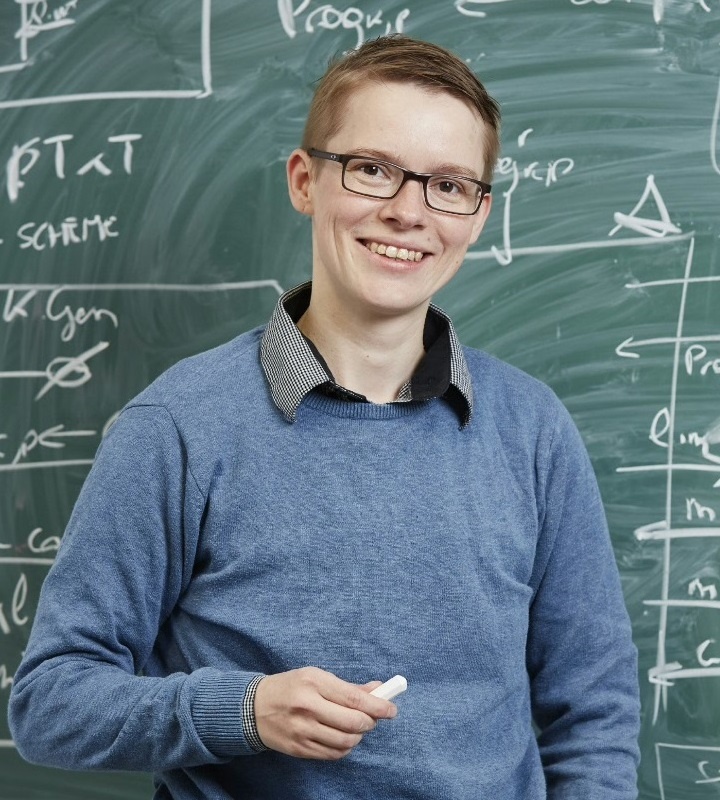
\includegraphics[height=2.5cm,keepaspectratio]{chris}
			
			\medskip
			\scriptsize
			\textbf{Chris Brzuska}
			
			Hamburg University of Technology

		\end{column}
		\begin{column}{0.49\textwidth}
			\centering
			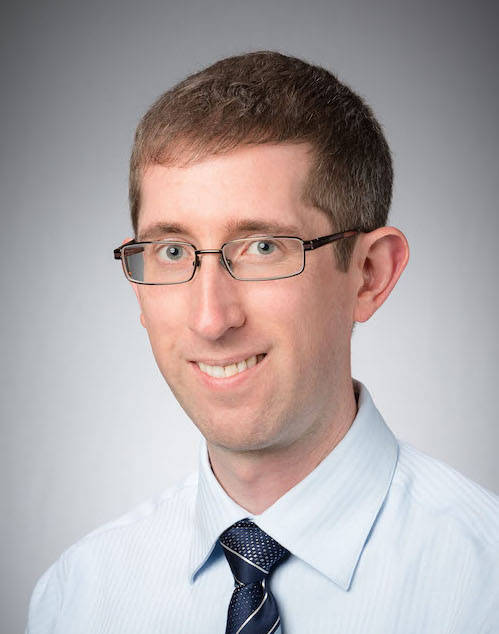
\includegraphics[height=2.5cm,keepaspectratio]{douglas}
			
			\medskip
			\scriptsize
			\textbf{Douglas Stebila}
			
			McMaster University, Hamilton

		\end{column}
	\end{columns}
\end{frame}





\section{AKE models}
\subsection{ake models}





\begin{frame}{Our formal security model}

	\vspace*{-0.5cm}

	Extended Bellare-Rogaway model adapted from \cite{EC:BelPoiRog00}
	
	\vspace*{\baselineskip}
	\uncover<2->{Adversary $\A$ can:}
	
	
	
	\begin{columns}
%	\hspace*{0.5cm}

		\begin{column}{0.45\textwidth}  %%<--- here
			\small

			\begin{itemize}
				\item<2-> Control all network communication
				
				\item[]
			
			
				\item<3-> Learn session keys $\ub{sk}$
								
				\item[]
				
				
				\item<4-> Learn long-term keys 
				
				\item[]
				
				\item<5-> \emph{Cannot} learn internal randomness 
			\end{itemize}
		\end{column}
		\hspace*{-0.5cm}
		\begin{column}{0.55\textwidth}
			\vspace*{-0.6cm}
%			\fbox{%
				\includegraphics[trim={1.3cm 2cm 1.4cm 1.4cm},clip,width=\textwidth]{tikz_KE_model}
%			}
		\end{column}
	
	\end{columns}
	
	
\end{frame}

\begin{frame}{Authenticated key exchange (AKE) security goals}
	\begin{itemize}
		\item \textbf{Key-secrecy:} attacker should learn nothing about $\ub{sk}$ for a \emph{fresh} session {\Large$\oracle{{\scriptscriptstyle\ub{U}}}$}
								
		
		\item[]
		
		\item \textbf{Authentication:} $\ub{sk}$ should only be shared with {\Large$\oracle{{\scriptscriptstyle\ub{U}}}$}'s intended peer
		 
		\item[]
	
		\item<2-> \textbf{Key-confirmation:} the intended peer \emph{actually} computed $\ub{sk}$
		
%		(also called \textbf{explicit entity authentication})
		
%		\item[]
%	
%		\item<2->
%		Model(s): three-party analogue of extended Canetti-Krawczyk model (eCK) without randomness reveal:
%			\begin{itemize}
%				\item[] \makebox[1.5cm][l]{AKE} -- full forward secrecy 
%				\item[] \makebox[1.5cm][l]{AKE$^w$} -- weak forward secrecy
%				\item[] \makebox[1.5cm][l]{AKE$^{\mathsf{static}}$} -- no forward secrecy
%			\end{itemize}

	
	\end{itemize}
\end{frame}


%\begin{frame}{Summary of formal key exchange models}
%	\begin{itemize}
%		\item The adversary controls all communication, i.e., it can:
%		
%		\begin{itemize}
%			\item observe all messages
%			\item reorder messages
%			\item drop messages
%			\item change messages
%			\item replay messages
%			\item change messages
%		\end{itemize} 
%		
%		\item Can run multiple sessions in parallel between multiple parties
%		
%		\item[]
%		
%		\item Can learn all keys except for the Test-session
%		
%		\item[]
%		
%		\item \textbf{Security goal}: distinguish the session key of the Test-session
%		from a completely random key
%		
%	\end{itemize}
%\end{frame}



\begin{frame}{Forward secrecy}

	\begin{figure}
		\centering
		\begin{tikzpicture}
			\draw[very thick] (0,0) -- (1,0);
			\draw[line width=5pt] (1,0) -- node[yshift=-8pt] (P) {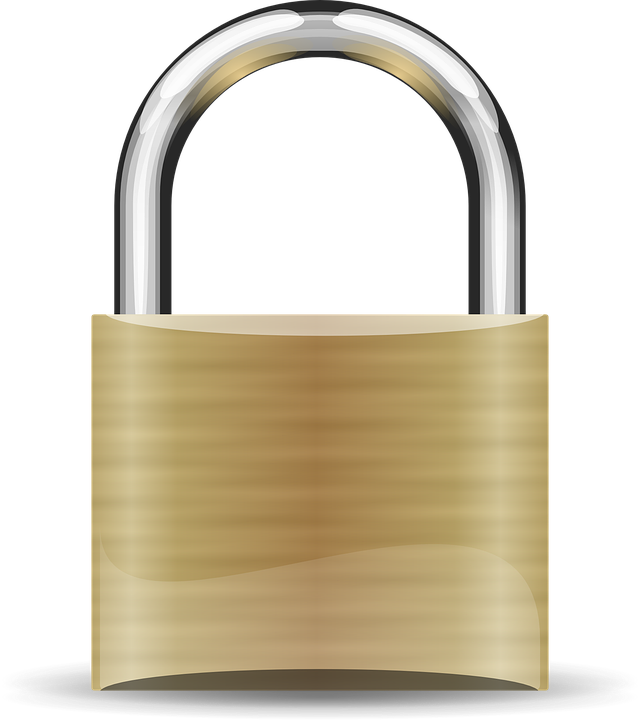
\includegraphics[width=0.08\textwidth]{padlock}} (2,0);
			\draw[very thick] (2,0) -- node[pos=0.6] (E) {
\includegraphics[width=0.1\textwidth]{explosion}}  (4,0);
			\draw[-triangle 60,very thick] (4,0) -- (4.6,0);
			\draw[-triangle 60,red!50!black] (3.1,0.4) to [bend left=-60] (1.5,0.4);
			\node[yshift=-6pt] at (P) {\Large$\oracle{{\scriptscriptstyle\ub{U}}}$};
		\end{tikzpicture}
	\end{figure}
	
	\vspace*{-0.2cm}


	\begin{itemize}
		\item Loss of a long-term key should not compromise \emph{previously} established session keys
		
		\item[]
		
		\uncover<2->{
		\begin{itemize}
		
		\item[]
		
		\item<2-> \textbf{Full} forward secrecy: adversary $\A$ can get long-term keys after {\Large$\oracle{{\scriptscriptstyle\ub{U}}}$} completed 
		
		\item[]
		
		\item<4-> \textbf{Weak} forward secrecy: $\A$ can get long-term keys after {\Large$\oracle{{\scriptscriptstyle\ub{U}}}$} completed---but only if $\A$ was \emph{passive}
		
		\item[]
		
		\item<3-> \textbf{No} forward secrecy: $\A$ cannot get long-term keys
		\end{itemize}
		}
	\end{itemize}
	
	\note{Lavabit, Edward Snowden}
\end{frame}



\begin{frame}<1-5>{Main results}
	\begin{enumerate}
		\item<1-> EAP is a secure 3P-AKE protocol with \emph{weak} forward secrecy
		
		\item[]
		
		\item<2-> EAP + key-confirmation is a secure 3P-AKE protocol with  \emph{full} forward secrecy
		
		\item[]
		
		\item<3-> EAP-TLS is a secure 2P-AKE protocol (with \emph{full} forward secrecy)
		
		\item[]
		
		\item<4-> 802.11 handshake protocol (WPA2-PSK) is a secure 2P-AKE protocol with \emph{no} forward secrecy
		
		\item[]
		
		\item<5-> WPA2-Enterprise is a secure 
		
		3P-AKE protocol with \emph{full} 
		 
		full secrecy
	\end{enumerate}		

	\vspace*{-1.5cm}
	\hfill
	\includestandalone[trim={1.1cm 2.8cm 1.1cm 2cm},clip,width=6cm,keepaspectratio]{tikz_EAP_and_802_11_mini}
	
	\vspace*{0.3cm}
\end{frame}




\begin{frame}{Our results -- caveats}
	
	\begin{itemize}
		\item Being ``secure'' is not an unconditional statement
		
		\item[]
		
		\item All results are relative to our \emph{model} of the protocol and relies on various assumptions
		
		\item[] 
		
		\item Model might not completely cover practice
	\end{itemize}
\end{frame}

\section{EAP}
\subsection{eap}


\miniframesoff
\begin{frame}
	\usebeamerfont*{frametitle} 
	\usebeamercolor[fg]{frametitle}
	
	\vfill
	\vfill
	\vfill
	\centering
	Extensible Authentication Protocol (EAP)
	\vfill
	\vfill
	\vfill
\end{frame}
\miniframeson


\begin{frame}{Extensible Authentication Protocol (EAP)}
	\begin{itemize}
		\item Generic authentication framework underlying WPA2-Enterprise
		
		\item[]
		
		\item<2-> Specifies:
		
		\begin{enumerate}
			\item<2-> a three-party architecture consisting of a \textbf{client}, a \textbf{server} and an \textbf{authenticator}

		
			\item<3-> a way of encapsulating concrete authentication mechanisms inside \textbf{EAP methods}
			
			\vspace*{0.2cm}
			\visible<4->{
				\begin{columns}
					\begin{column}{0.3\textwidth}
						\begin{itemize}
							\setlength\itemsep{-3pt}
							\item EAP-TLS
							\item EAP-TTLS
							\item EAP-IKEv2
							\item EAP-PWD
							\item EAP-PSK
						\end{itemize} 
					\end{column}
					
					\begin{column}{0.31\textwidth}
						\begin{itemize}
							\setlength\itemsep{-3pt}
							\item EAP-SIM
							\item EAP-AKA
							\item EAP-GTC
							\item PEAP
							\item LEAP
						\end{itemize} 
					\end{column}
					
					\begin{column}{0.3\textwidth}
						\begin{itemize}
							\setlength\itemsep{-3pt}
							\item EAP-FAST
							\item EAP-POTP
							\item EAP-EKE
							\item EAP-MD5
							\item ...
						\end{itemize} 
					\end{column}
				\end{columns}
			}	
			
		\end{enumerate}
	\end{itemize}		
\end{frame}



\begin{frame}{EAP framework}
	\begin{figure}
		\centering
		\includegraphics[page=2,trim={2cm 1cm 1cm 2cm},clip,width=0.78\textwidth]{tikz_EAP_and_802_11_mini}
	\end{figure}
\end{frame}





\miniframesoff
\begin{frame}
	\usebeamerfont*{frametitle} 
	\usebeamercolor[fg]{frametitle}
	
	\vfill
	\vfill
	\vfill
	\centering
	Composition Theorem 1
	\vfill
	\vfill
	\vfill
\end{frame}
\miniframeson


%\begin{frame}{Composition Theorem 1}
%	\centerline{
%		\includegraphics[page=1,width=0.98\textwidth]{tikz_EAP}
%	}
%\end{frame}



\begin{frame}<2->[b]{Modeling EAP without key-confirmation}
	\frametitle<3-5>{An attack}
%	\frametitle<6>{How to resolve?}
	\frametitle<6-10>{Channel binding}
	\frametitle<11>{Composition Theorem 1}
	
	\begin{overlayarea}{\textwidth}{0.6\textheight}
		\begin{figure}
			\centering
			\includestandalone[trim={1.1cm 2.2cm 1.2cm 1.5cm},clip,width=0.69\textwidth]{tikz_composition_1_simplified}
		\end{figure}
	\end{overlayarea}
	
	
	\vspace*{0.5cm}
	\uncover<11>{
		\textbf{Theorem 1:} EAP is a secure 3P-AKE protocol with \emph{weak} forward secrecy
	}
	\vspace*{0.5cm}
	
\end{frame}


%\miniframesoff
%\begin{frame}
%	\begin{center}
%		\usebeamerfont*{frametitle} 
%		\usebeamercolor[fg]{frametitle}
%		Composition Theorem 1 -- proof
%	\end{center}
%\end{frame}
%\miniframeson

%\begin{frame}{Composition Theorem 1 -- proof}
%	\centerline{
%		\includestandalone[width=0.95\textwidth]{tikz_composition_1_proof}
%	}
%\end{frame}


\miniframesoff
\begin{frame}
	\usebeamerfont*{frametitle} 
	\usebeamercolor[fg]{frametitle}
	
	\centering
	
	\vfill
	\vfill
	\vfill
	Composition Theorem 2
	\vfill
	\vfill
	\vfill
\end{frame}
\miniframeson


\begin{frame}[b]{Composition Theorem 2}
%	\vspace*{-1cm}

	\begin{overlayarea}{\textwidth}{0.7\textheight}%
		\begin{figure}
		\centering%
		\includegraphics<1>[page=1,trim={2cm 3cm 1.1cm 2cm},clip,width=0.78\textwidth]{tikz_EAP_and_802_11_mini}%
		\includegraphics<2>[page=2,trim={2cm 3cm 1.1cm 2cm},clip,width=0.78\textwidth]{tikz_EAP_and_802_11_mini}%
		\includegraphics<3->[page=6,trim={2cm 3cm 1.1cm 2cm},clip,width=0.78\textwidth]{tikz_EAP_and_802_11_mini}%
%		\includegraphics<3>[page=5,trim={2cm 3cm 1.5cm 2cm},clip,width=0.75\textwidth]{tikz_EAP_and_802_11_mini}%
		\end{figure}
	\end{overlayarea}

	\uncover<4->{%
		\textbf{Theorem 2:} EAP + key-confirmation is a secure 3P-AKE protocol with \emph{full} forward secrecy
	}
	\vspace*{0.4cm}
\end{frame}



\section{EAP-TLS}
\subsection{eap-tls}


\miniframesoff
\begin{frame}
	\usebeamerfont*{frametitle} 
	\usebeamercolor[fg]{frametitle}
	
	\centering
	
	\vfill
	\vfill
	\vfill		
	EAP-TLS
	\vfill
	\vfill
	\vfill
\end{frame}
\miniframeson




%\begin{frame}{TLS 1.2 handshake}
%	\centerline{
%		\includestandalone[width=\textwidth]{tikz_TLS_initial}	
%	}
%\end{frame}

\begin{frame}{EAP-Transport Layer Security}

	\vspace*{0.5cm}
	\begin{overlayarea}{\textwidth}{0.7\textheight}
		\begin{figure}
			\centering
			\includegraphics<1>[page=2,trim={1cm 3cm 1cm 2cm},clip,width=0.86\textwidth]{tikz_EAP_and_802_11_mini}%
			\includegraphics<2>[page=7,trim={1cm 3cm 1cm 2cm},clip,width=0.86\textwidth]{tikz_EAP_and_802_11_mini}%	
			\includegraphics<3>[page=8,trim={1cm 3cm 1cm 2cm},clip,width=0.86\textwidth]{tikz_EAP_and_802_11_mini}%
			\includegraphics<4>[page=9,trim={1cm 3cm 1cm 2cm},clip,width=0.86\textwidth]{tikz_EAP_and_802_11_mini}%	
		\end{figure}
	\end{overlayarea}
	\vspace*{-1cm}
	\begin{itemize}
		\item<4> EAP-TLS = certificate-based TLS encapsulated inside EAP 
	\end{itemize}
	\vspace*{4cm}
\end{frame}



\begin{frame}{Proving that EAP-TLS is a secure 2-party AKE protocol}
	
	
	\begin{itemize}
		\item<1-> Idea: modify existing \emph{proofs} of TLS to work for EAP-TLS
		
		\item[] 
		
		\item<2-> Problem: not modular
		
		\item[]
		
		\item<3-> Alternative: use existing \emph{results} on TLS to prove EAP-TLS
		
		\item[]
		
		\item<4-> Problem: TLS is \textbf{not} a secure authenticated key exchange (AKE) protocol,
		but rather a secure \textbf{channel establishment} protocol
		
	\end{itemize}
		
\end{frame}




\begin{frame}{Authenticated and Confidential Channel Establishment (ACCE)  protcols \cite{C:JKSS12}}
	\begin{itemize}
		\item All-in-one-definition: authenticated key exchange (AKE) protocol + encryption algorithm
	
		\item[]
		
		\item \textbf{Security goal:} session key established by the AKE should be safe to use for encryption algorithm
		
		\item[]
			
		\item Less stringent requirement than AKE
		
		\item[]
		
		\item \emph{Many} results showing that TLSv1.2 is a secure ACCE protocol (\cite{C:JKSS12,C:KraPatWee13,EPRINT:KohSchSch13,BrzuskaFSWW:2012:less_is_more,PKC:LSYKS14})
	\end{itemize}	
		
\end{frame}



\begin{frame}[c]{Our result}
	\centering
	\only<1>{``A secure ACCE $\implies$ a secure AKE''}	
	\only<2>{
		\begin{flushleft}
		\hspace*{0.7cm}	\textbf{Theorem 3:} 
		\end{flushleft}
		\vspace*{-0.1cm}
		\begin{equation*}
			\begin{array}{cc}
				\text{a secure \ub{TLS-like} ACCE protocol} & \\
				+ &   \\
				\text{a \textcolor{BurntOrange}{key-collision resistant} KDF} &  \Longrightarrow \text{a secure AKE}\\
				+ &  \\
				\text{a \ua{random oracle}} & \\
			\end{array}
		\end{equation*}}	
\end{frame}





%%%%%%%%%%%%%%%%%%%%%%%%%%%%%%%%%%%%%%%%%%%%


\section{802.11}
\subsection{ieee 802.11}

\miniframesoff
\begin{frame}
	\usebeamerfont*{frametitle} 
	\usebeamercolor[fg]{frametitle}
	
	\centering
	
	\vfill
	\vfill
	\vfill
	IEEE 802.11
	\vfill
	\vfill
	\vfill
\end{frame}
\miniframeson

\begin{frame}{IEEE 802.11}

	\begin{overlayarea}{\textwidth}{0.7\textheight}
		\begin{figure}
			\centering
			\includegraphics<1>[page=2,trim={1cm 3cm 1cm 2cm},clip,width=0.85\textwidth]{tikz_EAP_and_802_11_mini}%
			\includegraphics<2>[page=4,trim={1cm 3cm 1cm 2cm},clip,width=0.85\textwidth]{tikz_EAP_and_802_11_mini}%	
		\end{figure}
	\end{overlayarea}

\end{frame}

\begin{frame}{Wi-Fi Protected Access 2 (WPA2)}
	\begin{itemize}
		\item Protocol used to protect Wi-Fi networks
		
%		\item[]
%		
%		\item Very widely used -- more than 380 million Wi-Fi networks worldwide 
%		according to \url{https://wigle.net/}
		
		\item[]
		
		\item<1-> Consists of:
			\begin{enumerate}
				\item<1-> a 2-party key exchange protocol (4-Way Handshake)
				
				\item[]
				
				\item<1-> an encryption algorithm (CCMP)
				
				\item[]
				
				\item<1-> \alt<2>{\redout{a group key exchange protocol}}{a group key exchange protocol}
			\end{enumerate}
		
	\end{itemize}		
\end{frame}

\begin{frame}[label=4WHS]{802.11 4-Way Handshake (WPA2-PSK)}
	\begin{figure}
		\centering
		\includegraphics[trim={1cm 5cm 1.3cm 0},clip,width=0.8\textwidth]{tikz_4WHS}%
	\end{figure}
	\visible<2->{
		\textbf{Theorem 4:} The 4-Way Handshake is a secure 2P-AKE protocol with \emph{no} forward secrecy
	}
\end{frame}




\begin{frame}<2-10>{Putting it all together: WPA2-Enterprise}

	\begin{figure}
		\centering
%		\fbox{
		\includestandalone[trim={1cm 3cm 1cm 2cm},clip,width=0.95\textwidth]{tikz_EAP_and_802_11}%
%		}
	\end{figure}
	
	\visible<10->{
		\textbf{Theorem:} WPA2-Enterprise is a secure 3P-AKE protocol with \emph{full} forward secrecy
	}	
\end{frame}



\begin{frame}{KRACK attack on WPA2}
	
	\centering
	\begin{tikzpicture}
		\uncover<1->{
			\node[xshift=-1.2cm,yshift=0.5cm,inner sep=0] (bbc) {
				{\alt<4->{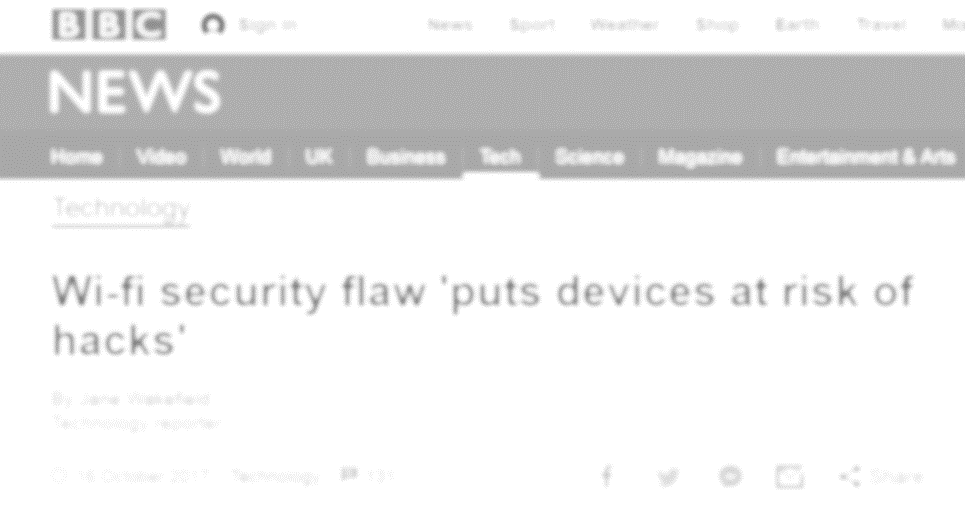
\includegraphics[width=0.5\textwidth]{krack_bbc_grey}}
						{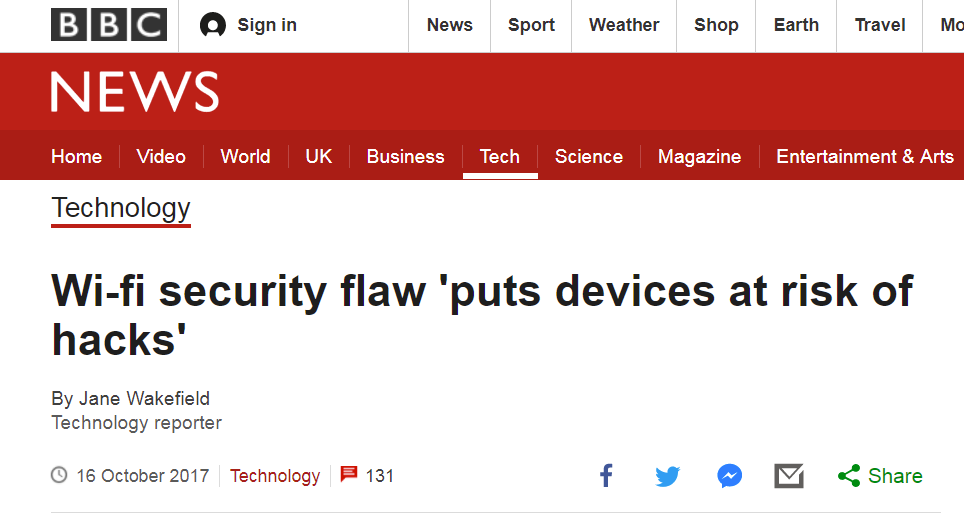
\includegraphics[width=0.5\textwidth]{krack_bbc}}}
			};
		}
		\uncover<2->{
			\node[xshift=1.2cm,yshift=0.4cm,inner sep=0] (bbc) {
				{\alt<4->{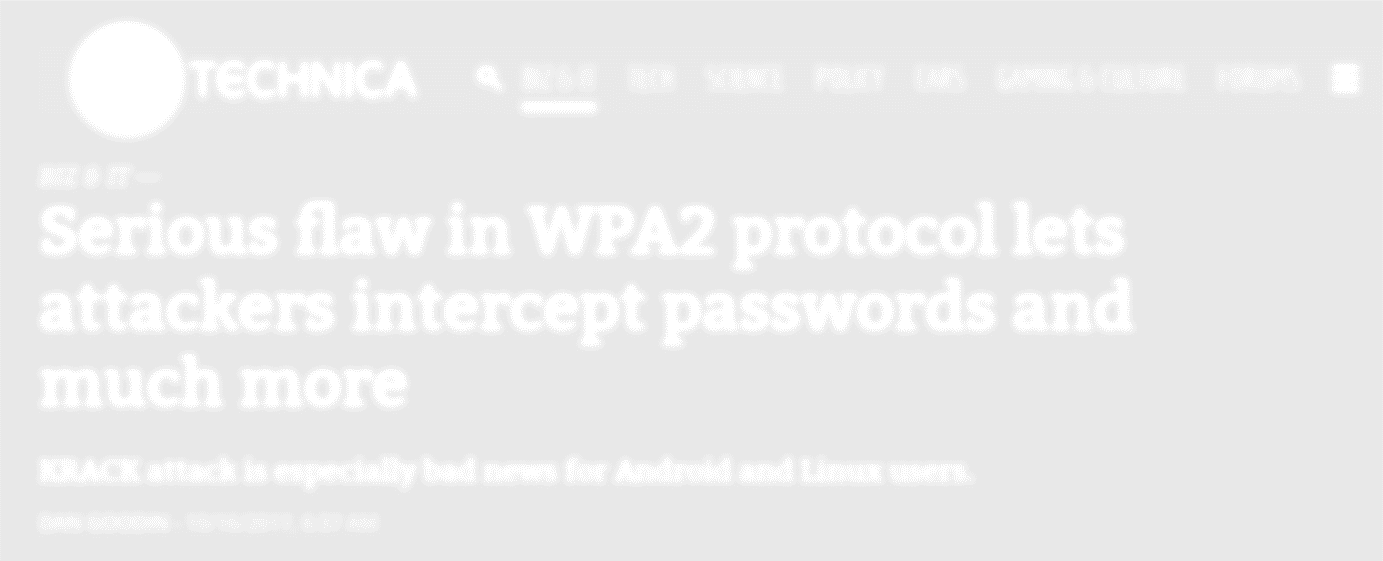
\includegraphics[width=0.5\textwidth]{krack_ars_grey}}
						{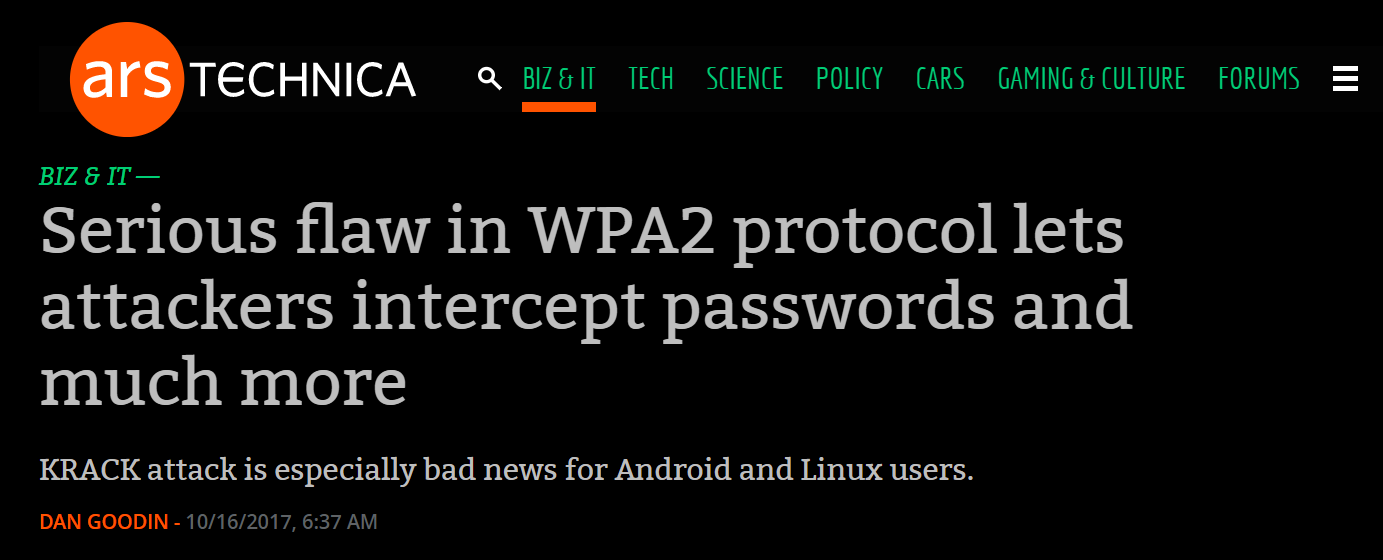
\includegraphics[width=0.5\textwidth]{krack_ars}}}
			};
		}
		\uncover<3->{
			\node[xshift=0.2cm,yshift=-1.7cm,inner sep=0] (bbc) {
				{\alt<4->{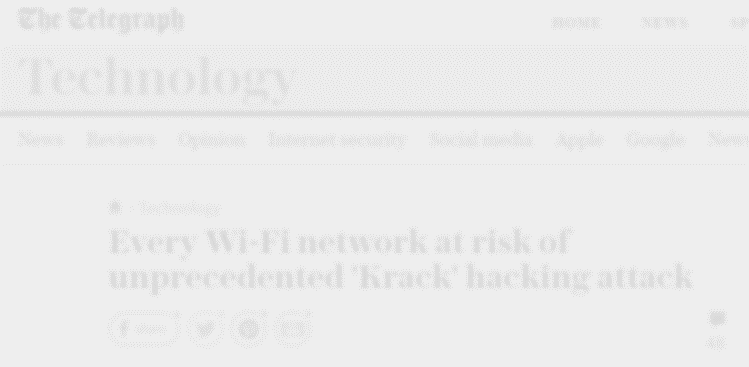
\includegraphics[width=0.5\textwidth]{krack_telegraph_grey}}
						{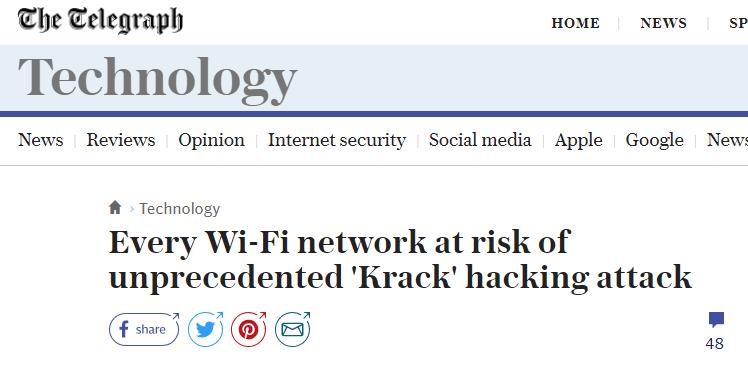
\includegraphics[width=0.5\textwidth]{krack_telegraph}}}
			};
		}
		\uncover<4->{
			\node[xshift=0cm,yshift=0cm,inner sep=0,draw,thick] (telegraph) {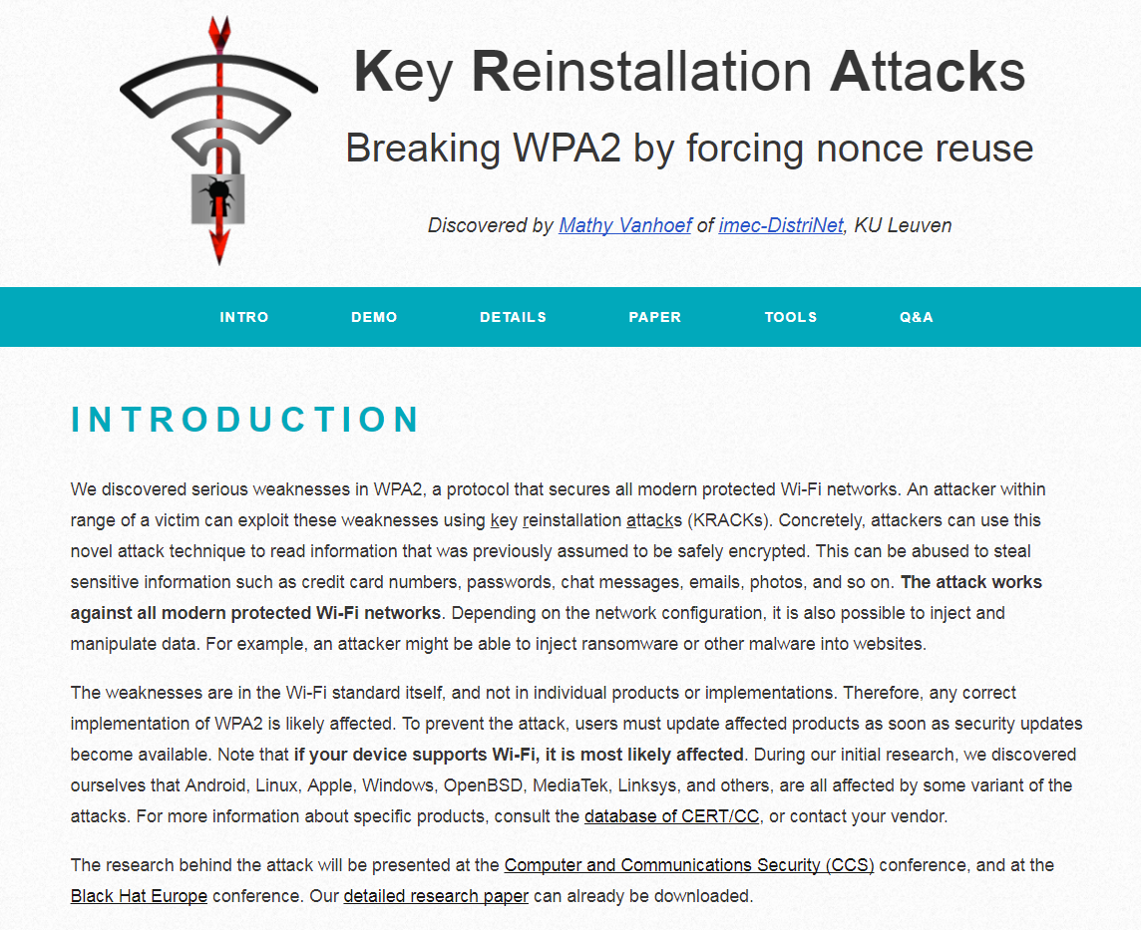
\includegraphics[width=0.6\textwidth]{KRACK}};
		}
	\end{tikzpicture}


\end{frame}

\begin{frame}{KRACK and our results}
	\begin{itemize}
	\item Does not invalidate our proofs
	
	\item[]
	
	\item Attack does not break the key exchange protocol (4-Way Handshake) nor the encryption algorithm (CCMP) \emph{individually},
	but rather when \emph{combined}
	
	\item[]
	
	\item Points out a discrepancy between our formal model and the real-world protocol
	
	\item[]
	
	\item<2> After patches, real-world protocol is now in line with our model!
	\end{itemize}
\end{frame}

\section{}


\begin{frame}{The end}
	\begin{center}
		Thank you
	\end{center}
\end{frame}

%\appendix
%
%\miniframesoff
%
%\backupbegin
%
%\begin{frame}[allowframebreaks]
\bibliographystyle{alpha}
\bibliography{../customrefs,../cryptobib/abbrev3,../cryptobib/crypto}
%\end{frame}
%
%\backupend

\end{document}